\documentclass[11pt,a4paper]{article}

\usepackage[utf8]{inputenc}
\usepackage[T1]{fontenc}
\usepackage[margin=2.4cm]{geometry}
\usepackage{mathpazo}
\usepackage{amsmath,amssymb,amsthm,bm}
\usepackage{enumitem}
\usepackage{booktabs,array,tabularx}
\usepackage{microtype}
\usepackage[most]{tcolorbox}
\usepackage{tikz}
\usepackage{float}
\usetikzlibrary{arrows.meta,positioning,calc,shapes.geometric,fit,backgrounds}
\usepackage{pgfplots}
\pgfplotsset{compat=1.17}
\usepackage[colorlinks=true,linkcolor=blue!50!black,urlcolor=blue!50!black]{hyperref}

\tikzset{>=Stealth}
\setlist{itemsep=2pt,topsep=4pt}
\setlength{\parindent}{0pt}
\setlength{\parskip}{5pt}

% ---------- theorem-like environments (amsthm) wrapped in boxes ----------
\theoremstyle{definition}
\newtheorem{definition}{Definition}[section]
\newtheorem{example}[definition]{Example}
\newtheorem{algorithm}[definition]{Algorithm}
\theoremstyle{plain}
\newtheorem{theorem}[definition]{Theorem}
\newtheorem{lemma}[definition]{Lemma}
\newtheorem{proposition}[definition]{Proposition}
\newtheorem{corollary}[definition]{Corollary}
\theoremstyle{remark}
\newtheorem*{remark}{Remark}

\tcbset{formalbox/.style={enhanced jigsaw,breakable,sharp corners,boxrule=0.6pt,
  left=6pt,right=6pt,top=4pt,bottom=4pt,before skip=10pt,after skip=8pt}}
\tcolorboxenvironment{definition}{formalbox,colback=black!3,colframe=black!60}
\tcolorboxenvironment{algorithm}{formalbox,colback=green!4,colframe=green!40!black}
\tcolorboxenvironment{example}{formalbox,colback=orange!5,colframe=orange!60!black}
\tcolorboxenvironment{theorem}{formalbox,colback=red!3,colframe=red!55!black}
\tcolorboxenvironment{lemma}{formalbox,colback=red!3,colframe=red!55!black}
\tcolorboxenvironment{proposition}{formalbox,colback=red!3,colframe=red!55!black}
\tcolorboxenvironment{corollary}{formalbox,colback=red!3,colframe=red!55!black}

\newtcolorbox{intuition}{enhanced jigsaw,breakable,colback=blue!6,colframe=blue!55!black,
  coltitle=white,fonttitle=\bfseries\sffamily,title={Intuition},boxrule=0.6pt,arc=2pt,
  left=6pt,right=6pt,top=4pt,bottom=4pt,before skip=8pt,after skip=12pt}

\newcommand{\slides}[1]{\par\vspace{-2pt}\noindent\emph{(slides #1)}\par\smallskip}

% ---------- notation ----------
\DeclareMathOperator{\atantwo}{atan2}
\newcommand{\E}{\mathbb{E}}
\newcommand{\R}{\mathbb{R}}
\newcommand{\hq}{\hat{\bm q}}
\newcommand{\cov}{\operatorname{cov}}
\newcommand{\robot}[3][fill=white]{\begin{scope}[shift={(#2)},rotate=#3]\draw[#1,thick] (0.24,0)--(-0.16,0.15)--(-0.16,-0.15)--cycle;\end{scope}}

\title{\textbf{Autonomous and Mobile Robotics}\\[4pt]
\Large Localization: Landmark-Based and SLAM\\[4pt]
\large Lecture notes}
\author{Prof.\ Giuseppe Oriolo --- Sapienza Universit\`a di Roma}
\date{Lecture of 9 November 2026}

\begin{document}
\maketitle
\tableofcontents
\bigskip

% =====================================================================
\section{Introduction and Recap: From Kalman Filters to Localization}
\slides{1}

In the previous chapter we met the \emph{Kalman filter} (KF) and its extension to nonlinear systems, the \emph{Extended Kalman Filter} (EKF). Both estimate the \emph{state} and the \emph{state covariance} of a system that is affected by
\begin{itemize}
  \item \textbf{process noise} (the model is not perfect, the commanded motion is not exactly executed), and
  \item \textbf{measurement noise} (the sensors are not ideal).
\end{itemize}
In this chapter we show how to turn this filter into actual \emph{localization methods}. As usual, the \textbf{unicycle} is the case study; only in the SLAM part will we switch to a simpler point robot. The roadmap is:
\begin{enumerate}[label=\arabic*.]
  \item EKF localization with \emph{distinguishable} landmarks (known identity),
  \item EKF localization with \emph{undistinguishable} landmarks (data association),
  \item EKF localization on a known \emph{metric map} (scan comparison),
  \item EKF \textbf{SLAM}: the map is unknown and is estimated together with the robot,
  \item the limits of Gaussian filters (kidnapped robot, multiple hypotheses).
\end{enumerate}

\paragraph{Notation.} The robot configuration is $\bm q=(x,\,y,\,\theta)^T$ and the inputs are the driving and steering velocities $(v,\omega)$. To avoid clashes with the velocity $v$, process noise is denoted by $\bm n_k$ (covariance $\bm N_k$) and measurement noise by $\bm w_k$ (covariance $\bm W_k$). A hat denotes an estimate, and $\hat{\bm q}_{k+1|k}$ is the estimate of $\bm q_{k+1}$ computed with the information available up to step $k$ (the \emph{prediction}, or ``intermediate estimate'').

\begin{definition}[Noisy nonlinear system for the EKF]
\label{def:system}
\[
\bm q_{k+1}=\bm f(\bm q_k,\bm u_k)+\bm n_k,\qquad 
\bm y_k=\bm h(\bm q_k)+\bm w_k ,
\]
where $\bm n_k\sim\mathcal N(\bm 0,\bm N_k)$ and $\bm w_k\sim\mathcal N(\bm 0,\bm W_k)$ are white, zero-mean Gaussian noises. If $\bm f$ and $\bm h$ are linear the KF applies; otherwise the equations must be \emph{linearized} and the EKF is used.
\end{definition}

\begin{algorithm}[EKF recursion]
\label{alg:ekf}
Given $\hq_{k|k}$ and $\bm P_{k|k}$:
\begin{enumerate}[label=\textbf{\arabic*.},leftmargin=1.6em]
  \item \textbf{Prediction.} $\hq_{k+1|k}=\bm f(\hq_{k|k},\bm u_k)$, \quad $\bm P_{k+1|k}=\bm F_k\bm P_{k|k}\bm F_k^T+\bm N_k$, \quad with $\bm F_k=\left.\dfrac{\partial\bm f}{\partial\bm q}\right|_{\bm q=\hq_{k|k}}$.
  \item \textbf{Innovation.} $\bm\nu_{k+1}=\bm y_{k+1}-\bm h(\hq_{k+1|k})$, \quad $\bm S_{k+1}=\bm H_{k+1}\bm P_{k+1|k}\bm H_{k+1}^T+\bm W_{k+1}$, \quad with $\bm H_{k+1}=\left.\dfrac{\partial\bm h}{\partial\bm q}\right|_{\bm q=\hq_{k+1|k}}$.
  \item \textbf{Correction.} $\bm K_{k+1}=\bm P_{k+1|k}\bm H_{k+1}^T\bm S_{k+1}^{-1}$, \quad $\hq_{k+1|k+1}=\hq_{k+1|k}+\bm K_{k+1}\bm\nu_{k+1}$, \quad $\bm P_{k+1|k+1}=(\bm I-\bm K_{k+1}\bm H_{k+1})\bm P_{k+1|k}$.
\end{enumerate}
When $\bm f(\bm q,\bm u)=\bm A\bm q+\bm B\bm u$ and $\bm h(\bm q)=\bm C\bm q$, this is exactly the (linear) KF with $\bm F=\bm A$, $\bm H=\bm C$.
\end{algorithm}

\begin{intuition}
The filter is a \emph{predict--then--correct} loop. Odometry tells us where we \emph{should} be (prediction, uncertainty grows because of $\bm N_k$); the sensor tells us what we \emph{actually see}; the difference $\bm\nu$ (the \emph{innovation}) is the ``surprise''. The matrix $\bm S$ says how big a surprise is normal, and the gain $\bm K$ decides how much of the surprise is believed.

A scalar toy case: prior variance $P=4$, sensor variance $W=1$, $H=1$. Then $S=5$ and $K=4/5=0.8$: the estimate moves 80\% of the way towards the measurement, because the sensor is four times more reliable than the prediction. If instead $W=16$ then $K=0.2$ and the measurement is mostly ignored.
\end{intuition}

% =====================================================================
\section{EKF Localization with Landmarks (Unicycle)}
\slides{2--10}

\subsection{Setting: range--bearing sensing of known landmarks}
\slides{2--4}

Let us start with a robot that localizes itself in an environment containing \textbf{landmarks}: easily recognizable elements that may be \emph{artificial} (placed on purpose) or \emph{natural} (objects already in the environment, such as doors or windows). We make the following assumptions.
\begin{itemize}
  \item A \textbf{unicycle-like} robot carries a sensor that measures the \textbf{range} (relative distance) and the \textbf{bearing} (relative orientation w.r.t.\ the sagittal axis) of certain landmarks.
  \item The landmark positions are \textbf{fixed and known}: in practice the robot owns a sort of map listing all landmark positions.
  \item Depending on the robot configuration, only a \textbf{subset} of the landmarks is actually visible at each time.
\end{itemize}
Suitable sensors are \emph{laser rangefinders} (LIDARs, with high angular resolution), \emph{depth cameras} (a depth value is attached to each pixel) and \emph{RFID sensors}.

\begin{figure}[H]
\centering
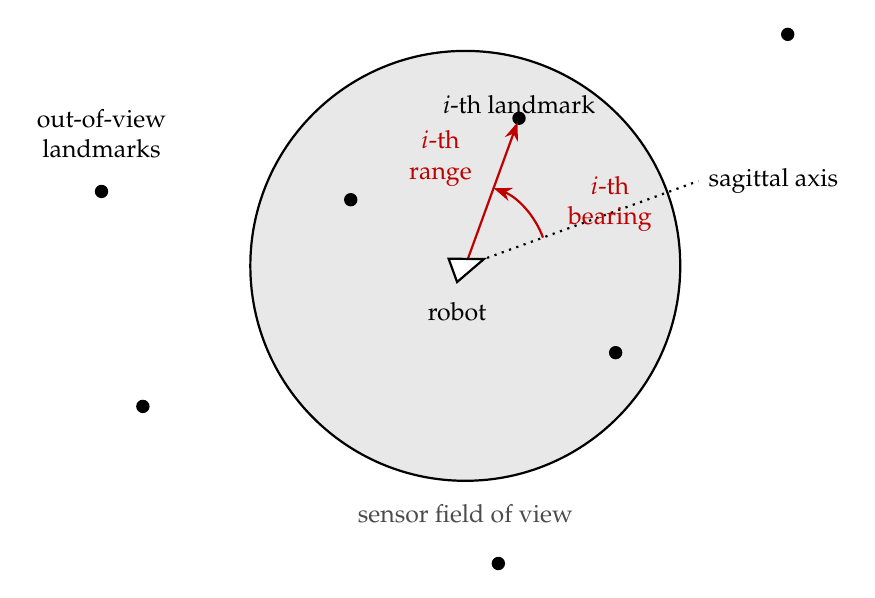
\begin{tikzpicture}[scale=1.05]
  \fill[gray!18] (0,0) circle (2.6);
  \draw[thick] (0,0) circle (2.6);
  \node[font=\small,gray!60!black] at (0,-3.0) {sensor field of view};
  % sagittal axis
  \draw[dotted,thick] (0,0) -- (20:3.0) node[right,font=\small] {sagittal axis};
  % landmarks in view
  \fill (70:1.9) circle (2.3pt) node[above,inner sep=1.5pt,font=\small] {$i$-th landmark};
  \fill (-30:2.1) circle (2.3pt);
  \fill (150:1.6) circle (2.3pt);
  % out of view
  \fill (-4.4,0.9) circle (2.3pt);
  \fill (-3.9,-1.7) circle (2.3pt);
  \fill (0.4,-3.6) circle (2.3pt);
  \fill (3.9,2.8) circle (2.3pt);
  \node[font=\small,align=center] at (-4.4,1.6) {out-of-view\\landmarks};
  % range and bearing
  \draw[->,red!75!black,thick] (0,0) -- (70:1.85);
  \node[red!75!black,font=\small,align=center] at (-0.3,1.3) {$i$-th\\range};
  \draw[->,red!75!black,thick] (20:1.0) arc (20:70:1.0);
  \node[red!75!black,font=\small,align=center] at (1.75,0.75) {$i$-th\\bearing};
  \robot{0,0}{20}
  \node[font=\small] at (-0.1,-0.55) {robot};
\end{tikzpicture}
\caption{Range--bearing sensing: only the landmarks inside the sensor field of view generate measurements. The bearing is measured from the sagittal axis of the robot.}
\label{fig:fov}
\end{figure}

\begin{intuition}
Think of a sailor taking bearings and distances to lighthouses whose positions are on the chart. One lighthouse already constrains the position to a circle (range) and fixes the heading once the position is known (bearing); two or more lighthouses pin everything down. The difficulty is not the geometry but the noise: odometry drifts, sensors are imprecise, and the EKF is the tool that blends the two optimally (under Gaussian assumptions).
\end{intuition}

\subsection{Model definition}
\slides{5--7}

\subsubsection*{Discretization of the process}
First of all we need a discretization of the kinematic model of the unicycle. The \emph{odometric equations} can be used as a discrete-time model of the robot; with the Euler method we obtain the following.

\begin{definition}[Discrete-time unicycle with process noise]
\label{def:process}
\[
\begin{cases}
x_{k+1}=x_k+v_k T_s\cos\theta_k+n_{1,k}\\
y_{k+1}=y_k+v_k T_s\sin\theta_k+n_{2,k}\\
\theta_{k+1}=\theta_k+\omega_k T_s+n_{3,k}
\end{cases}
\qquad\text{i.e.}\qquad
\bm q_{k+1}=\bm f(\bm q_k,\bm u_k)+\bm n_k ,
\]
with $\bm u_k=(v_k,\omega_k)^T$ and $\bm n_k=(n_{1,k},n_{2,k},n_{3,k})^T$ a \textbf{white Gaussian noise} with zero mean and covariance matrix $\bm N_k$.
\end{definition}

\begin{intuition}
Euler discretization simply says: ``in one sampling period the robot moves $v_kT_s$ along its current heading and turns by $\omega_kT_s$''. With $v=0.5$\,m/s, $\omega=0.2$\,rad/s and $T_s=0.1$\,s, each step is a 5\,cm advance and a $0.02$\,rad ($\approx1.15^\circ$) rotation. The noise $\bm n_k$ absorbs everything the model ignores (wheel slippage, encoder quantization, discretization error). Pure dead reckoning keeps adding these small errors, so the uncertainty of a prediction-only estimate grows without bound.
\end{intuition}

\subsubsection*{Landmarks and the association map}
Assume that $L$ landmarks are present, and denote by $(x_{\ell,i},y_{\ell,i})$ the position of the $i$-th one. The sensor cannot see all of them: let $L_k\le L$ be the number of landmarks the robot can \emph{actually} see at step $k$. Each of the $L_k$ measurements contains two components, a \emph{range} component (distance) and a \emph{bearing} component (angle of the landmark w.r.t.\ the sagittal axis).

For now we assume that, for each measurement, the \textbf{identity} of the observed landmark is known, i.e.\ landmarks are \emph{tagged} (e.g.\ by shape, color or radio frequency).

\begin{definition}[Association map]
\label{def:assoc}
Since landmarks are distinguishable, at each step $k$ we can build the map
\[
a:\{1,2,\dots,L_k\}\longmapsto\{1,2,\dots,L\},
\]
from measurements to landmarks: $a(i)$ is the \textbf{index of the landmark observed by the $i$-th measurement}.
\end{definition}

\begin{intuition}
The association map is just a ``who-is-who'' table. If the sensor returns three detections and reads their tags as ``landmark 7, landmark 2, landmark 5'', then $a(1)=7$, $a(2)=2$, $a(3)=5$ and $L_k=3$ even though $L$ may be $20$. Everything that follows hinges on this table being \emph{correct}: Section~\ref{sec:assoc} deals with what to do when it must be guessed.
\end{intuition}

\subsubsection*{Output equation: range and bearing}
Assume the sensor is mounted exactly at the contact point of the unicycle, so $(x_s,y_s)=(x_k,y_k)$. The range is simply the distance between the sensor and the landmark. Using the association map to select the landmark observed by the $i$-th measurement,
\[
\text{range}_i=\sqrt{(x_k-x_{\ell,a(i)})^2+(y_k-y_{\ell,a(i)})^2}.
\]
For the bearing, let $\gamma$ be the direction of the line of sight in the world frame, $\gamma=\atantwo(y_{\ell,a(i)}-y_k,\;x_{\ell,a(i)}-x_k)$. The bearing is measured from the sagittal axis, which points at angle $\theta_k$, hence $\beta=\gamma-\theta_k$ (Fig.~\ref{fig:bearing}).

\begin{figure}[H]
\centering
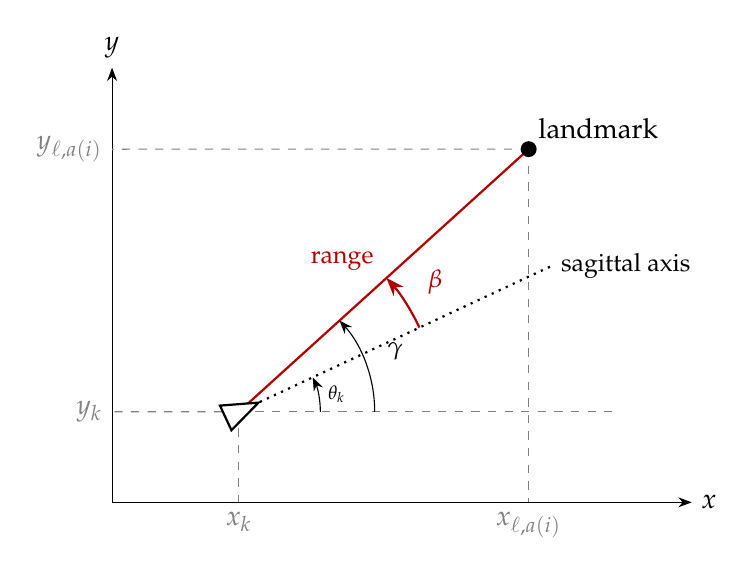
\begin{tikzpicture}[scale=1.15]
  \coordinate (R) at (1.4,1.0);
  \coordinate (L) at (4.6,3.9);
  \draw[->] (0,0) -- (6.4,0) node[right] {$x$};
  \draw[->] (0,0) -- (0,4.8) node[above] {$y$};
  \draw[dashed,gray] (R) -- ++(4.2,0);
  \draw[dashed,gray] (R) -- (R |- 0,0) node[below] {$x_k$};
  \draw[dashed,gray] (R) -- (0,1.0) node[left] {$y_k$};
  \draw[dashed,gray] (L) -- (L |- 0,0) node[below] {$x_{\ell,a(i)}$};
  \draw[dashed,gray] (L) -- (0,3.9) node[left] {$y_{\ell,a(i)}$};
  \draw[thick,dotted] (R) -- ++(25:3.8) node[right,font=\small] {sagittal axis};
  \draw[thick,red!70!black] (R) -- (L) node[midway,above left,font=\small] {range};
  \fill (L) circle (2.5pt) node[above right] {landmark};
  \draw[->] ($(R)+(0.9,0)$) arc (0:25:0.9) node[midway,right,font=\scriptsize] {$\theta_k$};
  \draw[->] ($(R)+(1.5,0)$) arc (0:42.2:1.5);
  \node[font=\small] at ($(R)+(21:1.85)$) {$\gamma$};
  \draw[->,red!70!black,thick] ($(R)+(25:2.2)$) arc (25:42.2:2.2);
  \node[red!70!black,font=\small] at ($(R)+(33.5:2.6)$) {$\beta$};
  \robot{1.4,1.0}{25}
\end{tikzpicture}
\caption{Geometry of the range--bearing measurement: $\gamma$ is the world-frame direction of the landmark, $\theta_k$ the robot heading, and $\beta=\gamma-\theta_k$ the measured bearing.}
\label{fig:bearing}
\end{figure}

\begin{definition}[Output equation of landmark-based localization]
\label{def:output}
The output is obtained by stacking the $L_k$ range--bearing pairs:
\[
\bm y_k=\bm h_k(\bm q_k,a)+\bm w_k=
\begin{pmatrix}\bm h_1(\bm q_k,a(1))\\ \vdots\\ \bm h_{L_k}(\bm q_k,a(L_k))\end{pmatrix}
+\begin{pmatrix}\bm w_{1,k}\\ \vdots\\ \bm w_{L_k,k}\end{pmatrix},
\]
where
\[
\bm h_i(\bm q_k,a(i))=
\begin{pmatrix}\text{range}_i\\ \text{bearing}_i\end{pmatrix}=
\begin{pmatrix}
\sqrt{(x_k-x_{\ell,a(i)})^2+(y_k-y_{\ell,a(i)})^2}\\[2pt]
\atantwo(y_{\ell,a(i)}-y_k,\;x_{\ell,a(i)}-x_k)-\theta_k
\end{pmatrix},
\]
and $\bm w_k=(\bm w_{1,k}^T\;\dots\;\bm w_{L_k,k}^T)^T$ is a \textbf{white Gaussian measurement noise} with zero mean and covariance $\bm W_k$.
\end{definition}

\begin{intuition}
A worked example. Robot at $\bm q=(0,0,\pi/2)$ (facing ``north''), landmark at $(3,4)$. The range is $\sqrt{9+16}=5$\,m. The line of sight points at $\gamma=\atantwo(4,3)\approx53.1^\circ$ while the robot faces $90^\circ$, so $\beta=53.1^\circ-90^\circ\approx-36.9^\circ$ ($-0.644$\,rad): the landmark appears $36.9^\circ$ to the \emph{right} of the nose (negative = clockwise). Note that the dimension of $\bm y_k$ is $2L_k$ and changes over time as landmarks enter or leave the field of view. In an implementation, the bearing component of the innovation must be wrapped to $(-\pi,\pi]$, otherwise a landmark seen at $+179^\circ$ and predicted at $-179^\circ$ looks like a $358^\circ$ error.
\end{intuition}

\subsection{Applying the EKF: linearization}
\slides{8--9}

We want to \emph{maintain} an accurate estimate of the robot configuration in the presence of process and measurement noise: this is the ideal setting for a Kalman filter. Actually, since \textbf{both} the process and the output equations are nonlinear, we must apply the \textbf{EKF}, and to do so the equations must be linearized.

\begin{proposition}[Linearized process]
\label{prop:F}
For the process of Definition~\ref{def:process},
\[
\bm F_k=\left.\frac{\partial\bm f}{\partial\bm q_k}\right|_{\bm q_k=\hq_k}=
\begin{pmatrix}
1&0&-v_kT_s\sin\hat\theta_k\\
0&1&v_kT_s\cos\hat\theta_k\\
0&0&1
\end{pmatrix}.
\]
\end{proposition}
\begin{proof}
Differentiate $\bm f=(x+vT_s\cos\theta,\;y+vT_s\sin\theta,\;\theta+\omega T_s)^T$ w.r.t.\ $(x,y,\theta)$: the first row is $(1,0,-vT_s\sin\theta)$, the second $(0,1,vT_s\cos\theta)$, the third $(0,0,1)$. Evaluate at $\hq_k$.
\end{proof}

\begin{intuition}
The identity part says that a position error stays a position error of the same size from one step to the next. The third column is the interesting one: a heading error $\delta\theta$ \emph{rotates the displacement}, so it turns into a position error $v_kT_s\,\delta\theta$ perpendicular to the motion. For $v_k=1$\,m/s, $T_s=0.1$\,s, $\hat\theta=\pi/2$: $\bm F_k$ has entry $-0.1$ in position $(1,3)$ and $0$ in $(2,3)$, i.e.\ a $1^\circ$ ($0.0175$\,rad) heading error induces a $1.75$\,mm sideways error per step; over many steps it compounds, which is why heading errors are the most dangerous ones in odometry.
\end{intuition}

\begin{proposition}[Linearized output]
\label{prop:H}
Let $\Delta x=x_{\ell,a(i)}-\hat x$, $\Delta y=y_{\ell,a(i)}-\hat y$ and $\rho^2=\Delta x^2+\Delta y^2$. The Jacobian of the $i$-th output, evaluated at the \emph{predicted} estimate, is
\[
\left.\frac{\partial\bm h_i}{\partial\bm q_k}\right|_{\bm q_k=\hq_{k+1|k}}=
\begin{pmatrix}
\dfrac{\hat x_{k+1|k}-x_{\ell,a(i)}}{\rho} & \dfrac{\hat y_{k+1|k}-y_{\ell,a(i)}}{\rho} & 0\\[10pt]
-\dfrac{\hat y_{k+1|k}-y_{\ell,a(i)}}{\rho^2} & \dfrac{\hat x_{k+1|k}-x_{\ell,a(i)}}{\rho^2} & -1
\end{pmatrix},
\]
with $\rho$ computed at $\hq_{k+1|k}$, and the full matrix is the vertical stack
$\bm H_{k+1}=\bigl((\partial\bm h_1/\partial\bm q)^T\;\cdots\;(\partial\bm h_{L_k}/\partial\bm q)^T\bigr)^T$.
\end{proposition}
\begin{proof}
\emph{First row} (range $\rho=\sqrt{(\hat x-x_\ell)^2+(\hat y-y_\ell)^2}$):
\[
\frac{\partial\rho}{\partial x}=\frac12\bigl[\cdots\bigr]^{-1/2}2(\hat x-x_\ell)=\frac{\hat x-x_\ell}{\rho},\qquad
\frac{\partial\rho}{\partial y}=\frac{\hat y-y_\ell}{\rho},\qquad
\frac{\partial\rho}{\partial\theta}=0 .
\]
\emph{Second row} (bearing $\beta=\operatorname{atan}(\Delta y/\Delta x)-\theta$, using $\tfrac{d}{du}\operatorname{atan}u=\tfrac1{1+u^2}$). Since $\partial\Delta x/\partial x=-1$,
\[
\frac{\partial\beta}{\partial x}=\frac{1}{1+\Delta y^2/\Delta x^2}\cdot\frac{\Delta y}{\Delta x^2}=\frac{\Delta y}{\rho^2}=-\frac{\hat y-y_\ell}{\rho^2},
\]
and since $\partial\Delta y/\partial y=-1$,
\[
\frac{\partial\beta}{\partial y}=\frac{1}{1+\Delta y^2/\Delta x^2}\cdot\Bigl(-\frac{1}{\Delta x}\Bigr)=-\frac{\Delta x}{\rho^2}=\frac{\hat x-x_\ell}{\rho^2},\qquad
\frac{\partial\beta}{\partial\theta}=-1 .
\]
The Jacobian is evaluated at $\hq_{k+1|k}$ because, at the moment of linearizing, the corrected estimate does not exist yet.
\end{proof}

\begin{intuition}
Read each entry as ``how the measurement changes if I nudge the robot''.
\begin{itemize}
  \item The range row is the \emph{unit vector from the landmark to the robot}, $(\hat x-x_\ell,\hat y-y_\ell)/\rho$: moving directly away from the landmark increases the range at rate $1$, moving sideways does not change it (to first order). The heading does not matter: entry $0$.
  \item The bearing row has the \emph{perpendicular} direction (scaled by $1/\rho$): moving sideways changes the viewing angle, and the effect shrinks with distance, because an offset of $1$\,m is a big angle at $2$\,m but a tiny one at $50$\,m. The $-1$ says that rotating the robot by $\delta$ rotates every bearing by $-\delta$.
\end{itemize}
Numerical example: robot estimate $(0,0,\pi/2)$, landmark $(3,4)$, so $\Delta x=3$, $\Delta y=4$, $\rho=5$. Then
\[
\bm H_i=\begin{pmatrix}-0.6&-0.8&0\\ 0.16&-0.12&-1\end{pmatrix}.
\]
If the sensor returns $\bm y_i=(5.1,\;-0.60)^T$ against the prediction $(5,\;-0.644)^T$, the innovation is $\bm\nu\approx(0.10,\;0.044)^T$: the landmark looks $10$\,cm farther than expected. Since $P\bm H^T\bm\nu$ is (for an isotropic $\bm P$) aligned with the range gradient $(-0.6,-0.8)$, the correction pushes the position estimate \emph{away from the landmark}, which is exactly what increases the predicted range.
\end{intuition}

\begin{algorithm}[EKF localization with tagged landmarks]
\label{alg:ekfloc}
At each step $k$:
\begin{enumerate}[label=\textbf{\arabic*.},leftmargin=1.6em]
  \item \emph{Predict} with odometry: $\hq_{k+1|k}=\bm f(\hq_{k|k},\bm u_k)$, $\;\bm P_{k+1|k}=\bm F_k\bm P_{k|k}\bm F_k^T+\bm N_k$ (Prop.~\ref{prop:F}).
  \item Read the $L_k$ visible landmarks and build the association map $a$ from their tags.
  \item Stack $\bm y_{k+1}$, compute the predicted output $\bm h(\hq_{k+1|k},a)$ and the matrix $\bm H_{k+1}$ (Prop.~\ref{prop:H}).
  \item \emph{Correct}: $\bm S$, $\bm K$, $\hq_{k+1|k+1}$, $\bm P_{k+1|k+1}$ as in Algorithm~\ref{alg:ekf}. If $L_k=0$ skip the correction (prediction only).
\end{enumerate}
\end{algorithm}

In short: once the linearization is available, we ``just crank the EKF engine''.

\subsection{Typical result}
\slides{10}

At the beginning we have no information about the state covariance, so the filter starts with an \textbf{isotropic Gaussian} (equal covariance in all directions). The nominal trajectory is a circle, but because of motion and measurement noise the \emph{actual} trajectory (ground truth) is different. Odometric localization alone drifts away, while the EKF estimate stays close to the ground truth.

\begin{figure}[H]
\centering
\begin{minipage}[t]{0.48\linewidth}
\centering
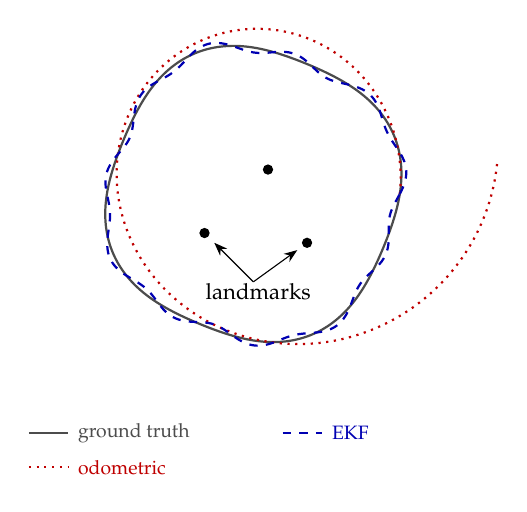
\begin{tikzpicture}[scale=0.62]
  \draw[black!70,thick,domain=0:360,samples=181,smooth,variable=\x]
    plot ({(3+0.12*sin(4*\x))*cos(\x)},{(3+0.12*sin(4*\x))*sin(\x)});
  \draw[red!75!black,thick,dotted,domain=0:360,samples=181,smooth,variable=\x]
    plot ({(3+0.8*\x/360)*cos(\x)+1.2*\x/360},{(3+0.8*\x/360)*sin(\x)+0.7*\x/360});
  \draw[blue!70!black,thick,dashed,domain=0:360,samples=181,smooth,variable=\x]
    plot ({(3+0.12*sin(4*\x)+0.1*sin(11*\x))*cos(\x)},{(3+0.12*sin(4*\x)+0.1*sin(11*\x))*sin(\x)});
  \foreach \x/\y in {0.3/0.5,-1.0/-0.8,1.1/-1.0}{\fill (\x,\y) circle (3pt);}
  \node[font=\footnotesize] at (0.1,-2.0) {landmarks};
  \draw[->] (0.0,-1.8) -- (0.9,-1.15);
  \draw[->] (0.0,-1.8) -- (-0.8,-1.0);
  % legend
  \draw[black!70,thick] (-4.6,-4.9) -- (-3.8,-4.9) node[right,font=\scriptsize] {ground truth};
  \draw[red!75!black,thick,dotted] (-4.6,-5.6) -- (-3.8,-5.6) node[right,font=\scriptsize] {odometric};
  \draw[blue!70!black,thick,dashed] (0.6,-4.9) -- (1.4,-4.9) node[right,font=\scriptsize] {EKF};
\end{tikzpicture}
\end{minipage}\hfill
\begin{minipage}[t]{0.48\linewidth}
\centering
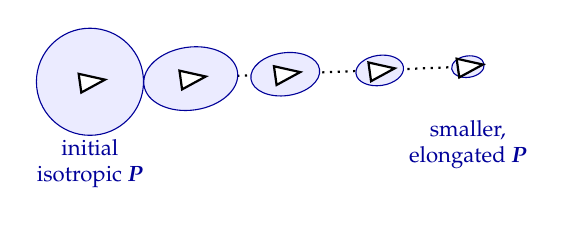
\begin{tikzpicture}[scale=0.8]
  \draw[dotted,thick] (0,0) -- (6.2,0.25);
  \draw[fill=blue!8,draw=blue!60!black] (0,0) circle (0.85);
  \draw[fill=blue!8,draw=blue!60!black,rotate around={8:(1.6,0.05)}] (1.6,0.05) ellipse (0.75 and 0.5);
  \draw[fill=blue!8,draw=blue!60!black,rotate around={8:(3.1,0.12)}] (3.1,0.12) ellipse (0.55 and 0.34);
  \draw[fill=blue!8,draw=blue!60!black,rotate around={8:(4.6,0.18)}] (4.6,0.18) ellipse (0.38 and 0.24);
  \draw[fill=blue!8,draw=blue!60!black,rotate around={8:(6.0,0.24)}] (6.0,0.24) ellipse (0.26 and 0.17);
  \foreach \x/\y in {0/0,1.6/0.05,3.1/0.12,4.6/0.18,6.0/0.24}{\robot{\x,\y}{8}}
  \node[font=\footnotesize,blue!60!black,align=center] at (0,-1.3) {initial\\isotropic $\bm P$};
  \node[font=\footnotesize,blue!60!black,align=center] at (6.0,-1.0) {smaller,\\elongated $\bm P$};
\end{tikzpicture}
\end{minipage}
\caption{Qualitative behaviour of EKF localization (schematic sketches, not experimental data). Left: nominal circular trajectory; the ground truth differs from it, odometry drifts away, the EKF stays near the ground truth. Right: the covariance ellipse of the position estimate starts large and isotropic and shrinks as landmark measurements are processed.}
\label{fig:typical1}
\end{figure}

\begin{intuition}
The ellipse is the $\bm P$ of the position estimate: a region where the robot probably is. With no prior it is a big circle. After a few range--bearing measurements the ellipse shrinks, and it becomes elongated along the directions that the landmarks constrain poorly (for example, along the line of sight, the \emph{bearing} constraint is weak at large distance). Odometry alone would have an ellipse that only grows; the measurements are what keep it bounded.
\end{intuition}

% =====================================================================
\section{EKF Localization with Undistinguishable Landmarks: Data Association}
\label{sec:assoc}
\slides{11--12}

Now we \textbf{remove the hypothesis} that the identity of each observed landmark is known: in practice landmarks can be \emph{undistinguishable} by the sensor (think of identical poles or door frames). Hence the association map must be \textbf{estimated} as well.

To estimate it we assume that, at the beginning of the EKF localization, the robot has a \emph{very good estimate} of state and covariance. To maintain a good estimate the EKF should pick the \emph{smallest} innovation: if the best candidate still produced a large innovation, the previous estimate would have been totally wrong. Therefore the basic idea is to associate each observation to the landmark that \textbf{minimizes the magnitude of the innovation} (\emph{nearest-neighbor association}).

\begin{definition}[Candidate innovation]
At step $k+1$ consider the $i$-th measurement $\bm y_{i,k+1}$ and compute \emph{all} the candidate innovations
\[
\bm\nu_{ij}=\bm y_{i,k+1}-\bm h_i(\hq_{k+1|k},j),\qquad j=1,\dots,L,
\]
where $\bm y_{i,k+1}$ is the \emph{actual} measurement and $\bm h_i(\hq_{k+1|k},j)$ is the \emph{expected} measurement if $\bm y_{i,k+1}$ referred to the $j$-th landmark.
\end{definition}

The smaller the innovation $\bm\nu_{ij}$, the more likely that the $i$-th measurement corresponds to the $j$-th landmark. However, we cannot measure the magnitude of $\bm\nu_{ij}$ with the classical Euclidean norm: the innovation must be \textbf{weighted with the uncertainty} of the measurement, which in the EKF is encoded in
\begin{definition}[Innovation covariance and association norm]
\[
\bm S_{ij}=\underbrace{\bm H_i(k+1,j)\,\bm P_{k+1|k}\,\bm H_i(k+1,j)^T}_{\text{uncertainty due to prediction}}+\underbrace{\bm W_{i,k+1}}_{\text{uncertainty due to sensor noise}},
\qquad
\chi_{ij}=\bm\nu_{ij}^T\bm S_{ij}^{-1}\bm\nu_{ij}.
\]
The estimated association map is
\[
a(i)=\arg\min_{j}\;\chi_{ij}.
\]
\end{definition}

\begin{algorithm}[Nearest-neighbor data association with gating and mutual exclusion]
For each measurement $i=1,\dots,L_k$ and each landmark $j=1,\dots,L$ compute $\bm\nu_{ij}$, $\bm S_{ij}$, $\chi_{ij}$. Then
\begin{itemize}
  \item \textbf{Nearest neighbor:} tentatively set $a(i)=\arg\min_j\chi_{ij}$.
  \item \textbf{Validation gating:} accept the pairing only if $\chi_{ij}$ is below a threshold $\gamma$; otherwise discard the measurement as spurious. (If $\bm\nu_{ij}$ is Gaussian with covariance $\bm S_{ij}$, $\chi_{ij}$ is $\chi^2$-distributed with $\dim\bm y_i=2$ degrees of freedom: $\gamma=5.99$ keeps $95\%$ of the correct pairings, $\gamma=9.21$ keeps $99\%$.)
  \item \textbf{Mutual exclusion:} two different measurements of the same scan cannot be assigned to the same landmark; in case of conflict keep the pairing with smaller $\chi$ and re-assign or discard the other.
\end{itemize}
The surviving pairs define $a$; then continue with the usual EKF correction.
\end{algorithm}

\begin{figure}[H]
\centering
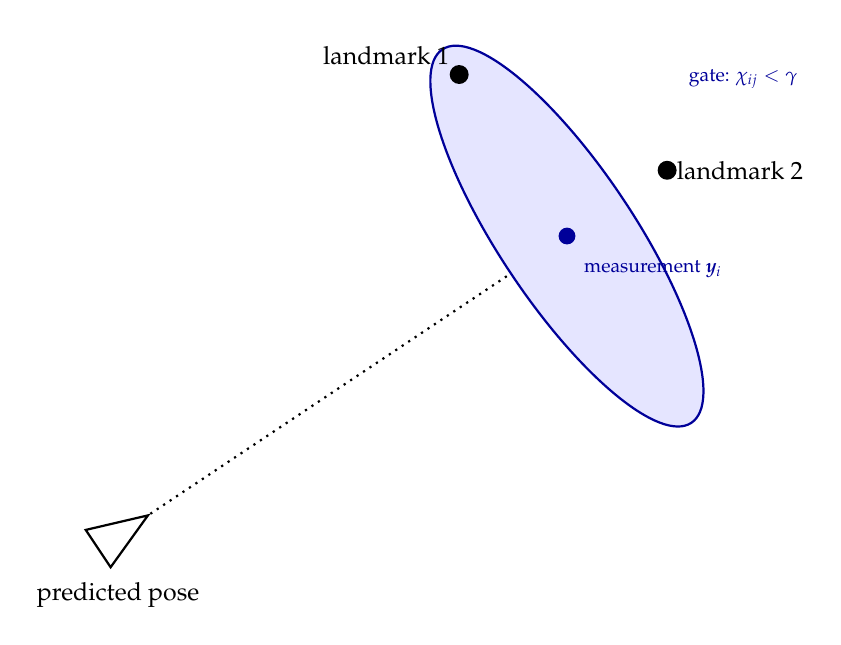
\begin{tikzpicture}[scale=1.9]
  \coordinate (Z) at (3.0,2.0);
  \draw[dotted,thick] (0,0) -- (Z);
  \robot{0,0}{33.7}
  \node[font=\small] at (0.0,-0.4) {predicted pose};
  \draw[fill=blue!10,draw=blue!60!black,thick,rotate around={123.7:(3.0,2.0)}] (3.0,2.0) ellipse (1.5 and 0.45);
  \fill[blue!60!black] (Z) circle (1.6pt);
  \node[blue!60!black,font=\scriptsize,anchor=north west] at (3.05,1.9) {measurement $\bm y_i$};
  \node[blue!60!black,font=\scriptsize,anchor=west] at (3.75,3.05) {gate: $\chi_{ij}<\gamma$};
  \fill (2.28,3.08) circle (1.8pt) node[above left,font=\small] {landmark 1};
  \fill (3.67,2.44) circle (1.8pt) node[right,font=\small] {landmark 2};
\end{tikzpicture}
\caption{Conceptual picture of validation gating (plane view). The ellipse is the region of $\bm S$-weighted compatibility around the measurement; it is long in the cross-range direction, where the bearing is uncertain, and short along the line of sight. Landmark~1 is farther from the measurement in Euclidean terms ($\approx1.3$) but inside the gate; landmark~2 is closer ($\approx0.8$) but outside.}
\label{fig:gating}
\end{figure}

\begin{intuition}
The Euclidean distance treats a $0.3$\,m error along a very precise range reading and a $0.3$\,m error in the cross-range direction (where a small bearing noise already causes decimeters of error) as equally bad. $\chi_{ij}$ measures instead \emph{how many standard deviations} away the candidate is --- the Mahalanobis distance --- so it forgives errors in directions where we are uncertain, and punishes errors in directions where we are sure.

Scalar toy example (range only): the measured range is $5.2$\,m; landmark~1 predicts $5.0$\,m ($\nu_{i1}=0.2$, $S=0.01$), landmark~2 predicts $4.9$\,m ($\nu_{i2}=0.3$, $S=0.09$). Euclidean: $0.2<0.3$, choose landmark~1. Weighted: $\chi_{i1}=0.2^2/0.01=4$, $\chi_{i2}=0.3^2/0.09=1$, so landmark~2 is the better explanation: a $0.2$\,m miss when we are confident to $\pm0.1$\,m is a $2\sigma$ event, while a $0.3$\,m miss with $\pm0.3$\,m accuracy is only $1\sigma$.

The price: a wrong association is not a harmless outlier, it feeds a plausible but false innovation to the filter. This is why the method needs a good initial estimate, and why gating and mutual exclusion are added ``in practice''.
\end{intuition}

% =====================================================================
\section{EKF Localization on a Map}
\slides{13--17}

\subsection{Metric maps}
\slides{13}

Now we \textbf{remove landmarks} and assume that a \textbf{metric map} $\mathcal M$ of the environment is known to the robot. This may be a \emph{line-based map} (walls and obstacles as segments, as in a floor plan) or an \textbf{occupancy grid}, where the environment is divided into cells that can be \textbf{white = free}, \textbf{black = occupied}, \textbf{gray = unknown}.

\begin{figure}[H]
\centering
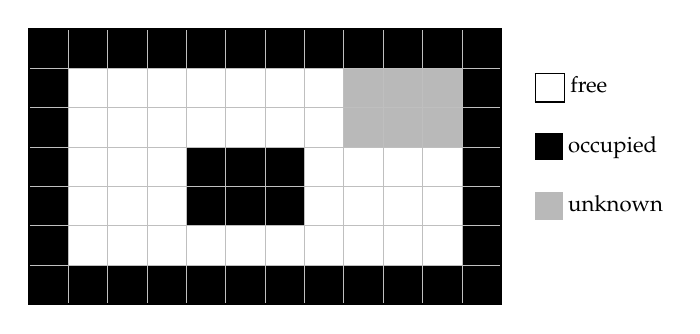
\begin{tikzpicture}[scale=0.5]
  \foreach \x in {0,...,11}{\foreach \y in {0,...,6}{
    \pgfmathtruncatemacro{\occ}{(\x==0||\x==11||\y==0||\y==6||(\x>=4&&\x<=6&&\y>=2&&\y<=3))?1:(((\x>=8&&\x<=10&&\y>=4&&\y<=5))?2:0)}
    \ifcase\occ \fill[white] (\x,\y) rectangle ++(1,1);
    \or \fill[black] (\x,\y) rectangle ++(1,1);
    \or \fill[gray!55] (\x,\y) rectangle ++(1,1);
    \fi
  }}
  \draw[gray!50,very thin] (0,0) grid (12,7);
  \draw[thick] (0,0) rectangle (12,7);
  \node[font=\footnotesize,anchor=west] at (12.6,5.5) {\fcolorbox{black}{white}{\phantom{x}} free};
  \node[font=\footnotesize,anchor=west] at (12.6,4.0) {\colorbox{black}{\phantom{x}} occupied};
  \node[font=\footnotesize,anchor=west] at (12.6,2.5) {\colorbox{gray!55}{\phantom{x}} unknown};
\end{tikzpicture}
\caption{A toy occupancy grid: a room with a central obstacle and a region never observed.}
\label{fig:grid}
\end{figure}

\subsection{Scan-based output and the innovation}
\slides{14--15}

The robot must \emph{scan} the environment to navigate in it: we assume it is equipped with a \textbf{range finder}, e.g.\ a laser sensor, whose typical scan is a fan of range readings with an \emph{uncertainty interval} on each reading. The idea is to use the \textbf{whole scan as output vector}: its components are the range readings in all available directions.

\begin{definition}[Scan-based innovation]
Let $\bm y_{k+1}$ be the actual scan and $\bm h(\hq_{k+1|k},\mathcal M)$ the \emph{predicted scan}, obtained by placing the robot at configuration $\hq_{k+1|k}$ in the map $\mathcal M$ and computing the range that each beam would read. The innovation is
\[
\bm\nu_{k+1}=\bm y_{k+1}-\bm h(\hq_{k+1|k},\mathcal M).
\]
\end{definition}

\begin{figure}[H]
\centering
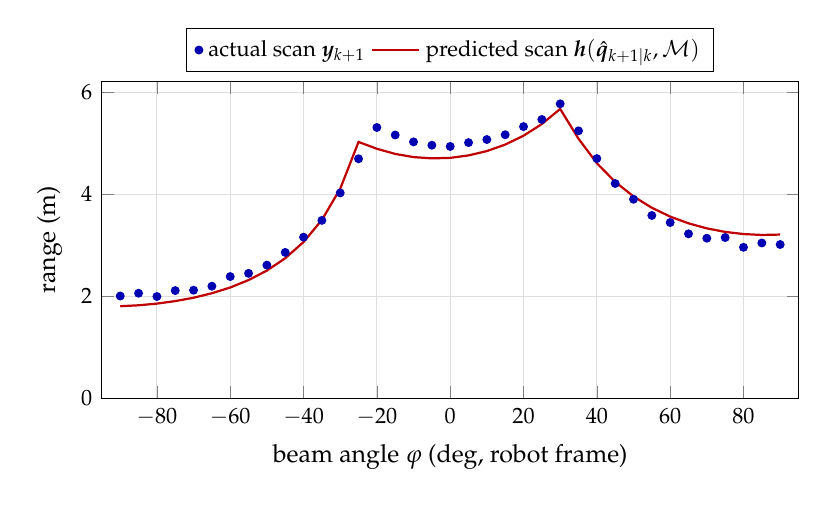
\begin{tikzpicture}
\begin{axis}[width=0.86\linewidth,height=5.6cm,xlabel={beam angle $\varphi$ (deg, robot frame)},ylabel={range (m)},
  xmin=-95,xmax=95,ymin=0,ymax=6.2,grid=both,grid style={gray!25},legend style={font=\footnotesize,at={(0.5,1.03)},anchor=south,legend columns=2},tick label style={font=\footnotesize},label style={font=\small}]
\addplot[only marks,mark=*,mark size=1.4pt,blue!70!black] coordinates {(-90,2.004) (-85,2.058) (-80,1.994) (-75,2.110) (-70,2.118) (-65,2.196) (-60,2.385) (-55,2.448) (-50,2.609) (-45,2.858) (-40,3.157) (-35,3.486) (-30,4.024) (-25,4.693) (-20,5.306) (-15,5.159) (-10,5.024) (-5,4.959) (0,4.935) (5,5.010) (10,5.070) (15,5.164) (20,5.324) (25,5.463) (30,5.770) (35,5.240) (40,4.697) (45,4.209) (50,3.900) (55,3.582) (60,3.444) (65,3.222) (70,3.136) (75,3.150) (80,2.958) (85,3.043) (90,3.013)};
\addlegendentry{actual scan $\bm y_{k+1}$}
\addplot[thick,red!75!black] coordinates {(-90,1.804) (-85,1.822) (-80,1.855) (-75,1.904) (-70,1.970) (-65,2.058) (-60,2.171) (-55,2.316) (-50,2.502) (-45,2.744) (-40,3.062) (-35,3.495) (-30,4.106) (-25,5.023) (-20,4.889) (-15,4.788) (-10,4.726) (-5,4.701) (0,4.711) (5,4.759) (10,4.844) (15,4.971) (20,5.145) (25,5.374) (30,5.669) (35,5.085) (40,4.607) (45,4.240) (50,3.955) (55,3.733) (60,3.560) (65,3.428) (70,3.329) (75,3.260) (80,3.218) (85,3.200) (90,3.208)};
\addlegendentry{predicted scan $\bm h(\hat{\bm q}_{k+1|k},\mathcal M)$}
\end{axis}
\end{tikzpicture}
\caption{Illustrative (synthetic) scan comparison in a rectangular room: the actual scan is taken from the true pose; the prediction is computed from a slightly wrong estimated pose ($30$\,cm and $20$\,cm position error, $4^\circ$ heading error). The innovation is the vertical gap between the two curves, beam by beam.}
\label{fig:scan}
\end{figure}

\begin{intuition}
Imagine groping in a dark room with a fan of whiskers: you know the floor plan, so for any guessed pose you can \emph{imagine} what your whiskers should feel. The innovation is the mismatch between the imagined and the felt ranges; the EKF moves the pose estimate in the direction that reduces the mismatch. With a laser of $1^\circ$ resolution over $180^\circ$ the output has $181$ components, much richer than a handful of landmarks, and no tags are needed.
\end{intuition}

\begin{definition}[Aliasing]
\emph{Aliasing} denotes ambiguities in the environment: different parts of it (or different poses) produce the same sensor view.
\end{definition}

Note that \textbf{no explicit landmark data association is needed}, but ambiguities in the environment may severely displace the estimate, leading to \emph{incorrect localization}. Since both the process dynamics (the robot kinematic model) and the output function $\bm h$ are nonlinear, we use the EKF to perform localization.

\begin{figure}[H]
\centering
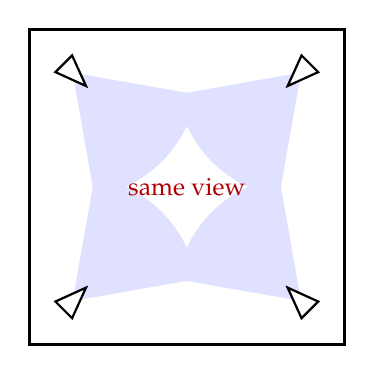
\begin{tikzpicture}
  \draw[very thick] (0,0) rectangle (4,4);
  \foreach \x/\y/\a in {0.55/0.55/45, 3.45/0.55/135, 3.45/3.45/225, 0.55/3.45/315}{
    \fill[blue!12] (\x,\y) -- ++(\a-35:1.6) arc[start angle=\a-35,end angle=\a+35,radius=1.6] -- cycle;
    \robot{\x,\y}{\a}
  }
  \node[red!70!black,font=\small] at (2,2) {same view};
\end{tikzpicture}
\caption{Aliasing in a perfectly square, empty room: the four poses are related by $90^\circ$ rotations and return identical scans; a scan comparison cannot tell them apart.}
\label{fig:aliasing}
\end{figure}

\begin{intuition}
Because the filter only compares ``what I see'' with ``what I should see from my believed pose'', any other pose that would see the same thing is an equally good explanation. A long featureless corridor is another classic case: the scan says nothing about the position \emph{along} the corridor. With a good prior the filter stays on the right hypothesis; if aliasing pulls it onto a wrong one, nothing in the innovation reveals the mistake.
\end{intuition}

\subsection{Architecture}
\slides{16}

\begin{figure}[H]
\centering
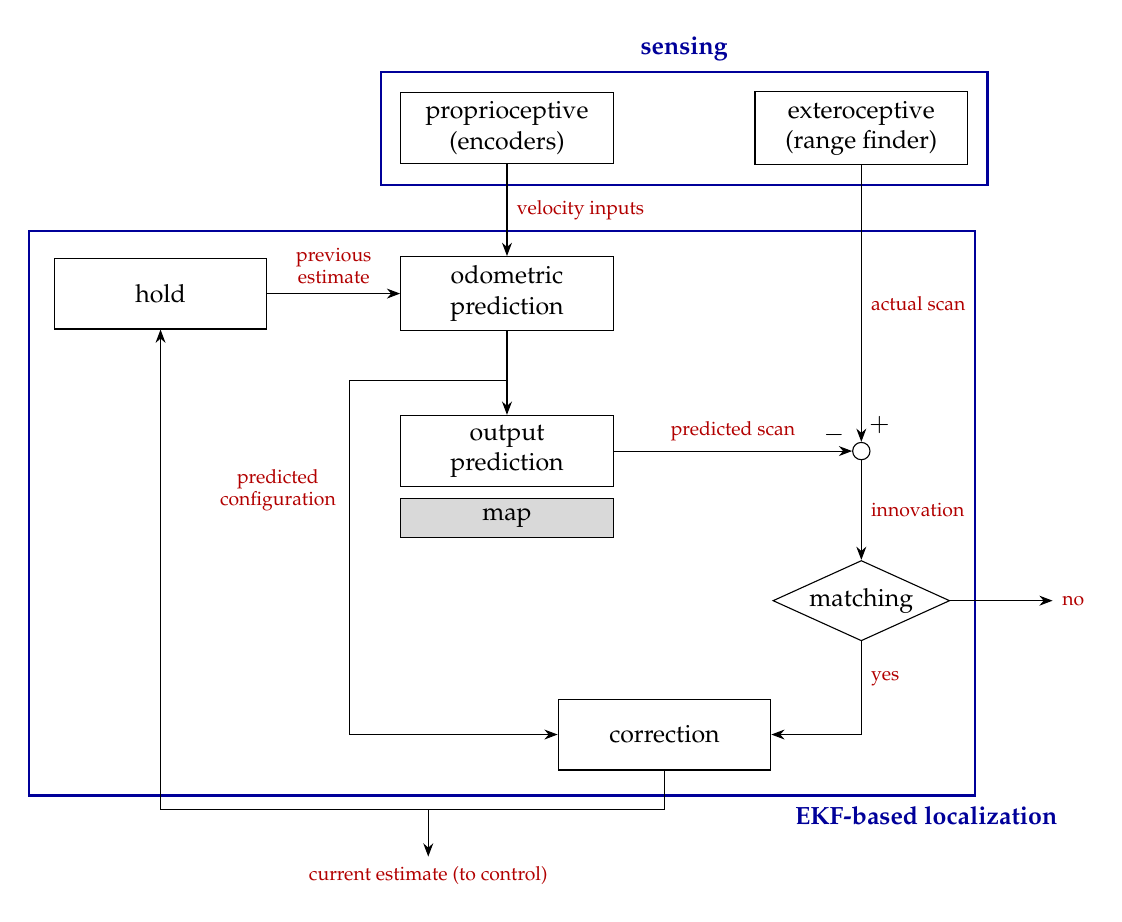
\begin{tikzpicture}[blk/.style={draw,rectangle,minimum width=2.7cm,minimum height=0.9cm,align=center,font=\small,fill=white},
  lab/.style={font=\scriptsize,red!70!black,align=center}]
  % sensing
  \node[blk] (enc) at (0,5.4) {proprioceptive\\(encoders)};
  \node[blk] (rf) at (4.5,5.4) {exteroceptive\\(range finder)};
  \begin{scope}[on background layer]
    \node[draw=blue!60!black,thick,fit=(enc)(rf),inner sep=7pt,label={[blue!60!black,font=\small\bfseries]above:sensing}] {};
  \end{scope}
  % EKF blocks
  \node[blk] (odo) at (0,3.3) {odometric\\prediction};
  \node[blk] (hold) at (-4.4,3.3) {hold};
  \node[blk] (outp) at (0,1.3) {output\\prediction};
  \node[blk,fill=gray!30,minimum height=0.5cm] (map) at (0,0.45) {map};
  \node[circle,draw,inner sep=1.5pt,font=\small] (sum) at (4.5,1.3) {$\;$};
  \node[diamond,draw,aspect=2.2,inner sep=1pt,font=\small] (match) at (4.5,-0.6) {matching};
  \node[blk] (corr) at (2.0,-2.3) {correction};
  \begin{scope}[on background layer]
    \node[draw=blue!60!black,thick,fit=(hold)(odo)(outp)(map)(sum)(match)(corr),inner sep=9pt,label={[blue!60!black,font=\small\bfseries]below right:EKF-based localization}] (ekf) {};
  \end{scope}
  % arrows
  \draw[->] (enc) -- (odo) node[midway,right,lab] {velocity inputs};
  \draw[->] (rf) -- (sum) node[midway,right,lab] {actual scan};
  \draw[->] (hold) -- (odo) node[midway,above,lab] {previous\\estimate};
  \draw[->] (odo) -- (outp);
  \draw[->] (0,2.2) -- (-2.0,2.2) |- (corr.west) ;
  \node[lab,anchor=east] at (-2.05,0.8) {predicted\\configuration};
  \draw[->] (outp) -- (sum) node[midway,above,lab] {predicted scan};
  \node[font=\small,above left=-1pt] at (sum.west) {$-$};
  \node[font=\small,above right=-1pt] at (sum.north) {$+$};
  \draw[->] (sum) -- (match) node[midway,right,lab] {innovation};
  \draw[->] (match.south) |- (corr.east) node[pos=0.2,right,lab] {yes};
  \draw[->] (match.east) -- ++(1.3,0) node[right,lab] {no};
  \draw[->] (corr.south) -- ++(0,-0.5) -| (hold.south);
  \draw[->] (-1.0,-3.25) -- ++(0,-0.6) node[below,lab] {current estimate (to control)};
\end{tikzpicture}
\caption{Architecture of EKF-based localization on a map. Odometry feeds the prediction; the predicted configuration is placed in the map to generate the predicted scan, which is compared with the actual one. If the innovation passes the matching test the correction is performed; if not, the correction is skipped and the previous estimate is retained. The current estimate closes the loop (hold) and is available to the control scheme.}
\label{fig:arch}
\end{figure}

The blocks are the following.
\begin{itemize}
  \item \textbf{Sensing:} a \emph{proprioceptive} sensor (wheel encoders, giving the velocity inputs) and an \emph{exteroceptive} sensor (the range finder, giving the actual scan).
  \item \textbf{Odometric prediction:} propagates the previous estimate (kept by the \emph{hold} block, a one-step memory) with the velocity inputs, producing the predicted configuration.
  \item \textbf{Output prediction:} uses the \textbf{map} to compute the predicted scan from the predicted configuration.
  \item \textbf{Scan comparison:} actual minus predicted scan gives the innovation; the \textbf{matching} block checks that it is compatible (as for gating); if so (\emph{yes}) the \textbf{correction} produces the current estimate, otherwise (\emph{no}) no correction takes place.
  \item The \textbf{current estimate} is what the control scheme uses.
\end{itemize}

\subsection{Typical result}
\slides{17}
\begin{figure}[H]
	\centering
	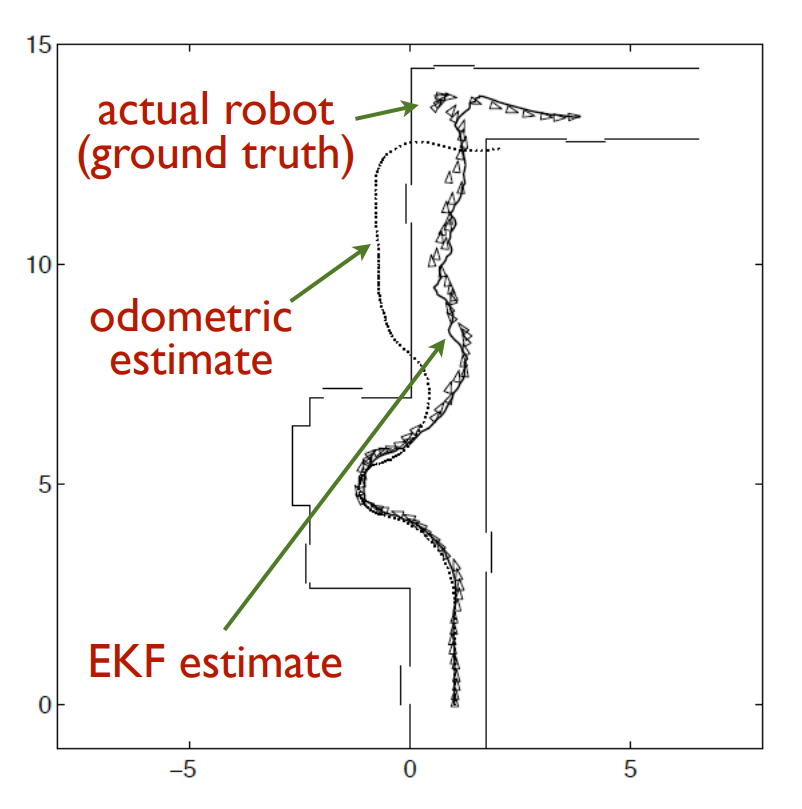
\includegraphics[width=0.7\linewidth]{1794219626005.png}
	\caption{The experiment shown in class concerns a \textbf{robotized wheelchair with high slippage}, equipped with \textbf{5 ultrasonic sensors with a 2\,Hz rate} (cheap sensors) and with a \emph{shadow zone} behind the robot where nothing is measured. The odometric estimate drifts substantially from the ground truth because of slippage, whereas the EKF estimate remains close to the actual trajectory.
}\label{fig:1794219626005}
\end{figure}

\begin{intuition}
This is the strongest argument for the method: the sensors are poor (few, slow, noisy), the odometry is bad (slippage), and yet combining a \emph{known map} with a Kalman filter yields a trajectory that tracks the ground truth. Neither source alone would suffice: odometry has no memory of absolute position, the sparse sonar readings have no memory of motion.
\end{intuition}

% =====================================================================
\section{EKF SLAM}
\slides{18--23}

\subsection{From localization to SLAM}
\slides{18}

Now we \textbf{remove the hypothesis that the environment is known a priori}: as it moves, the robot must use its sensors to \emph{build a map} and at the same time \emph{localize itself}. This task is called \textbf{SLAM}: \emph{Simultaneous Localization And Map-building}.

In \textbf{probabilistic SLAM} the idea is to \emph{estimate the map features in addition to the robot configuration}. Here we discuss a simple landmark-based version of the problem which can be solved using the KF or the EKF.

\begin{intuition}
It is the chicken-and-egg problem of exploration: to localize you need a map, to build the map you need to know where you are. Probabilistic SLAM resolves the circle by never committing: robot and landmark positions are all unknowns of a single estimation problem, each with its own uncertainty, refined together.
\end{intuition}

\subsection{Landmark-based SLAM with a point robot}
\slides{19--23}

The landmarks play the role of the map, so the goal is to estimate their positions. To work with the simplest problem we make the following assumptions.
\begin{itemize}
  \item \textbf{Omnidirectional point-robot:} its configuration is then just a Cartesian position.
  \item \textbf{$L$ landmarks, positions unknown:} they are distributed in the environment at unknown places.
  \item \textbf{Ideal sensor:} the robot can \emph{see}, \emph{identify} and \emph{measure} the relative position of \textbf{all} landmarks w.r.t.\ itself (infinite field of view, no occlusions).
\end{itemize}

\begin{definition}[Extended state]
\label{def:extstate}
The state to be estimated contains the robot \emph{and} the landmark positions:
\[
\bm x=\bigl(\underbrace{x\;\;y}_{\text{robot}}\;\;\underbrace{x_{\ell1}\;\;y_{\ell1}}_{\text{landmark }1}\;\;\dots\;\;\underbrace{x_{\ell L}\;\;y_{\ell L}}_{\text{landmark }L}\bigr)^T\in\R^{2+2L}.
\]
\end{definition}

\subsubsection*{Process equation}
Since the landmarks are fixed, the discrete-time model of the robot+landmarks system is the following (with $T_s=1$ without loss of generality).

\begin{proposition}[Linear process model of SLAM]
\label{prop:slamproc}
\[
\bm x_{k+1}=\bm x_k+
\begin{pmatrix}1&0\\0&1\\0&0\\0&0\\\vdots&\vdots\\0&0\\0&0\end{pmatrix}
\begin{pmatrix}u_{x,k}\\u_{y,k}\end{pmatrix}+
\begin{pmatrix}n_{x,k}\\n_{y,k}\\0\\0\\\vdots\\0\\0\end{pmatrix},
\]
where $\bm u_k=(u_{x,k},u_{y,k})^T$ are the robot velocity inputs and $\bm n_{xy,k}=(n_{x,k},n_{y,k})^T$ is a white Gaussian noise with zero mean and covariance $\bm N_{xy,k}$. This is a \textbf{linear} model
\[
\bm x_{k+1}=\bm A\bm x_k+\bm B\bm u_k+\bm n_k,\qquad \bm A=\bm I_{2+2L},\quad \bm B=\begin{pmatrix}\bm I_2\\\bm 0\end{pmatrix},
\]
with noise $\bm n_k=(n_{1,k}\;n_{2,k}\;\dots\;n_{2+2L,k})^T$ and covariance
\[
\bm N_k=\begin{pmatrix}\bm N_{xy,k}&\bm 0&\cdots&\bm 0\\\bm 0&\bm 0&\cdots&\bm 0\\\vdots&\vdots&\ddots&\vdots\\\bm 0&\bm 0&\cdots&\bm 0\end{pmatrix}.
\]
\end{proposition}

\begin{intuition}
Only the first two entries of the state move: the landmarks are fixed, so their rows of the dynamics are ``stay where you are'', and since there is nothing random about a landmark standing still, the process noise acts \emph{only on the robot block}. The landmarks can become more certain over time precisely because their prediction step adds no uncertainty. For $L=2$ the state has dimension $6$, $\bm B$ is $6\times2$ and $\bm N_k$ is a $6\times6$ matrix whose only non-zero block is the $2\times2$ upper-left one.
\end{intuition}

\subsubsection*{Output equation}
\begin{proposition}[Linear output of SLAM]
\label{prop:slamout}
The $i$-th measurement contains the relative position of the $i$-th landmark w.r.t.\ the sensor,
\[
\bm y_{i,k}=\begin{pmatrix}x_{\ell i,k}-x_k\\y_{\ell i,k}-y_k\end{pmatrix}+\bm w_{i,k}=\bm C_i\bm x_k+\bm w_{i,k},\qquad
\bm C_i=\begin{pmatrix}-1&0&0&\cdots&0&1&0&0&\cdots&0\\0&-1&0&\cdots&0&0&1&0&\cdots&0\end{pmatrix},
\]
where the first ``$1$'' sits in the $(2i+1)$-th column, $\bm w_{i,k}$ is white Gaussian with covariance $\bm W_{i,k}$. Stacking all measurements,
\[
\bm y_k=\bm C\bm x_k+\bm w_k,\quad
\bm C=\begin{pmatrix}\bm C_1\\\vdots\\\bm C_L\end{pmatrix},\quad
\bm w_k=\begin{pmatrix}\bm w_{1,k}\\\vdots\\\bm w_{L,k}\end{pmatrix},\quad
\bm W_k=\begin{pmatrix}\bm W_{1,k}&\bm 0&\cdots&\bm 0\\\bm 0&\bm W_{2,k}&\cdots&\bm 0\\\vdots&\vdots&\ddots&\vdots\\\bm 0&\bm 0&\cdots&\bm W_{L,k}\end{pmatrix}.
\]
\end{proposition}

\begin{algorithm}[KF-based SLAM]
With $\bm A=\bm I$, $\bm B$, $\bm C$, $\bm N_k$, $\bm W_k$ defined above, at each step: predict $\hat{\bm x}_{k+1|k}=\hat{\bm x}_{k|k}+\bm B\bm u_k$, $\bm P_{k+1|k}=\bm P_{k|k}+\bm N_k$; then correct with $\bm\nu=\bm y_{k+1}-\bm C\hat{\bm x}_{k+1|k}$, $\bm S=\bm C\bm P_{k+1|k}\bm C^T+\bm W_{k+1}$, $\bm K=\bm P_{k+1|k}\bm C^T\bm S^{-1}$ (Algorithm~\ref{alg:ekf} with $\bm F=\bm A$, $\bm H=\bm C$). At this point, we just crank the KF engine.
\end{algorithm}

\begin{remark}
We can use the \emph{linear} filter (KF) thanks to the assumptions of a \textbf{point robot} (no kinematic constraints, so the motion is linear in the inputs) and of measuring \textbf{directly positions} (no angles, hence no trigonometry in the output). For a unicycle with range--bearing sensing, the same SLAM problem would be nonlinear and need the EKF with the Jacobians of Section~2.
\end{remark}

\begin{figure}[H]
\centering
\begin{minipage}[t]{0.48\linewidth}
\centering
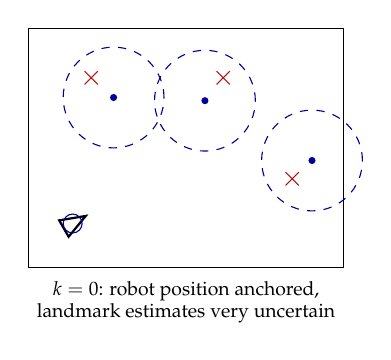
\begin{tikzpicture}[scale=0.8]
  \draw (0,0) rectangle (5,3.8);
  \foreach \x/\y/\dx/\dy in {1.0/3.0/0.35/-0.3, 3.1/3.0/-0.3/-0.35, 4.2/1.4/0.3/0.3}{
    \node[red!70!black] at (\x,\y) {$\times$};
    \fill[blue!60!black] (\x+\dx,\y+\dy) circle (1.6pt);
    \draw[dashed,blue!60!black] (\x+\dx,\y+\dy) circle (0.8);
  }
  \robot{0.7,0.7}{30}
  \draw[blue!60!black] (0.7,0.7) circle (0.15);
  \node[font=\scriptsize,align=center] at (2.5,-0.55) {$k=0$: robot position anchored,\\landmark estimates very uncertain};
\end{tikzpicture}
\end{minipage}\hfill
\begin{minipage}[t]{0.48\linewidth}
\centering
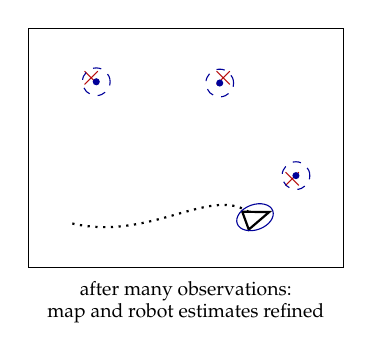
\begin{tikzpicture}[scale=0.8]
  \draw (0,0) rectangle (5,3.8);
  \foreach \x/\y/\dx/\dy in {1.0/3.0/0.08/-0.05, 3.1/3.0/-0.06/-0.07, 4.2/1.4/0.05/0.06}{
    \node[red!70!black] at (\x,\y) {$\times$};
    \fill[blue!60!black] (\x+\dx,\y+\dy) circle (1.6pt);
    \draw[dashed,blue!60!black] (\x+\dx,\y+\dy) circle (0.22);
  }
  \draw[dotted,thick] (0.7,0.7) .. controls (2,0.4) and (3,1.4) .. (3.6,0.8);
  \robot{3.6,0.8}{20}
  \draw[blue!60!black,rotate around={20:(3.6,0.8)}] (3.6,0.8) ellipse (0.3 and 0.2);
  \node[font=\scriptsize,align=center] at (2.5,-0.55) {after many observations:\\map and robot estimates refined};
\end{tikzpicture}
\end{minipage}
\caption{Qualitative sketch of EKF SLAM ($\times$ true landmark, dot estimated landmark, dashed circle uncertainty). The map is not given: it is estimated, and its uncertainty shrinks as the robot keeps observing the landmarks.}
\label{fig:slam}
\end{figure}

\begin{intuition}
Each measurement only gives the \emph{difference} $\bm\ell_i-\bm p$ between a landmark and the robot. In 1D: robot at $0$, landmark measured at $+5.1$\,m. That is compatible with ``robot $0$, landmark $5.1$'' as well as ``robot $10$, landmark $15.1$''. Relative measurements alone fix the \emph{shape} of the map, not its absolute placement; what anchors the whole picture is the \textbf{initial robot position}, which the filter treats as (nearly) known with a small prior covariance, while landmark priors are large. The covariance $\bm P$ becomes a full matrix with cross-terms: the errors of landmark estimates are \emph{correlated} through the robot position they were measured from, and when one landmark is refined the others benefit. The price is the size: the state has $2+2L$ entries and $\bm P$ has $(2+2L)^2$.
\end{intuition}

% =====================================================================
\section{How Realistic is KF/EKF Localization?}
\slides{24--25}

\begin{itemize}
  \item KF/EKF assume that the probability distribution of the state is \textbf{unimodal}, and in particular a \textbf{Gaussian}.
  \item This requires an \textbf{accurate estimate of the initial configuration} and \textbf{relatively small uncertainties}: this is the \emph{position tracking} problem.
  \item However, if the robot is released at an \textbf{unknown (or poorly known) position}, the probability distribution of the state becomes \textbf{multimodal} in the presence of aliasing: this is the \emph{kidnapped robot} problem.
\end{itemize}

\begin{figure}[H]
\centering
\newcommand{\gp}[3]{(#3*exp(-((\x-(#1))^2)/(2*#2*#2)))}
\newcommand{\wallstrip}[2]{%
  \draw[fill=red!10,draw=black!60] (0,#1) rectangle (8,#1+0.5);
  \foreach \dx in {1.5,2.6,5.6}{\draw[fill=brown!70!black] (\dx-0.15,#1) rectangle (\dx+0.15,#1+0.5);}
  \begin{scope}[shift={(#2,#1-0.02)}]\fill[red!80!black] (0,-0.12) circle (0.14);\end{scope}}
\begin{tikzpicture}[scale=0.82,x=1cm,y=1cm]
  % panel 1: no information
  \wallstrip{9.0}{1.5}
  \draw[->] (0,8.0) -- (8.3,8.0) node[right,font=\scriptsize] {$x$};
  \draw[very thick] (0,8.12) -- (8,8.12);
  \node[font=\scriptsize,anchor=east] at (-0.1,8.4) {bel$(x)$};
  % panel 2: sense a door
  \wallstrip{6.7}{1.5}
  \draw[->] (0,5.1) -- (8.3,5.1);
  \draw[red,thick,domain=0:8,samples=241,smooth,variable=\x] plot ({\x},{6.05+\gp{1.5}{0.1}{0.6}+\gp{2.6}{0.1}{0.6}+\gp{5.6}{0.1}{0.6}});
  \draw[->,gray] (0,6.05) -- (8.3,6.05);
  \node[font=\scriptsize,red,anchor=east] at (-0.1,6.35) {$p(z|x)$};
  \draw[thick,domain=0:8,samples=241,smooth,variable=\x] plot ({\x},{5.15+\gp{1.5}{0.1}{0.6}+\gp{2.6}{0.1}{0.6}+\gp{5.6}{0.1}{0.6}});
  \node[font=\scriptsize,anchor=east] at (-0.1,5.45) {bel$(x)$};
  % panel 3: move
  \wallstrip{3.6}{2.6}
  \draw[->] (0,2.5) -- (8.3,2.5);
  \draw[thick,domain=0:8,samples=241,smooth,variable=\x] plot ({\x},{2.55+\gp{2.6}{0.22}{0.3}+\gp{3.7}{0.22}{0.3}+\gp{6.7}{0.22}{0.3}});
  \node[font=\scriptsize,anchor=east] at (-0.1,2.85) {bel$(x)$};
  % panel 4: sense a door again
  \wallstrip{0.9}{2.6}
  \draw[->] (0,-0.2) -- (8.3,-0.2);
  \draw[thick,domain=0:8,samples=241,smooth,variable=\x] plot ({\x},{-0.15+\gp{2.6}{0.1}{1.15}+\gp{3.7}{0.2}{0.12}+\gp{6.7}{0.2}{0.12}});
  \node[font=\scriptsize,anchor=east] at (-0.1,0.2) {bel$(x)$};
  % panel 5: move on
  \wallstrip{-2.0}{4.0}
  \draw[->] (0,-3.1) -- (8.3,-3.1);
  \draw[thick,domain=0:8,samples=241,smooth,variable=\x] plot ({\x},{-3.05+\gp{4.0}{0.3}{0.55}+\gp{1.5}{0.3}{0.05}+\gp{7.0}{0.3}{0.05}});
  \node[font=\scriptsize,anchor=east] at (-0.1,-2.7) {bel$(x)$};
\end{tikzpicture}
\caption{One-dimensional kidnapped-robot example (a robot in a corridor with three doors; schematic redrawing). Top to bottom: no information (uniform belief); sensing a door makes the belief \textbf{multimodal} with three equal peaks; moving shifts and flattens them; sensing a door again reinforces the peak that matches a door; moving on leaves a single dominant hypothesis. A single Gaussian cannot represent the second panel.}
\label{fig:doors}
\end{figure}

For these problems one needs to \textbf{track multiple hypotheses}, and more general Bayesian estimators (e.g.\ \textbf{particle filters}) may be used.

\begin{intuition}
Put the robot down somewhere in a long corridor and let it see a door. It cannot know \emph{which} door: ``door~1 \emph{or} door~2 \emph{or} door~3'', three separate lumps of belief. A Gaussian has one lump only and would have to summarize them by a mean and a variance: with doors at $1.5$, $2.6$ and $5.6$\,m and equal belief, the mean is $\approx3.2$\,m --- a stretch of blank wall where the robot cannot even be, with a huge variance. The EKF is therefore excellent for \emph{tracking} (where we start nearly right and stay right) and unsuitable for \emph{global} localization. A particle filter keeps many weighted guesses (``particles'') of the pose, can hold several lumps at once, and prunes them as more doors are seen or non-doors are traversed, as in the figure.
\end{intuition}

% =====================================================================
\section{Summary}

\subsection{Comparison of the methods}

\begin{table}[ht]
\centering
\small
\renewcommand{\arraystretch}{1.25}
\newcolumntype{Y}{>{\raggedright\arraybackslash}X}
\begin{tabularx}{\linewidth}{@{}>{\raggedright\arraybackslash}p{2.4cm}YYYY@{}}
\toprule
\textbf{Method} & \textbf{Environment info} & \textbf{Measurement $\bm y$} & \textbf{Filter / association} & \textbf{Main limitation}\\
\midrule
EKF, tagged landmarks & landmark positions known, identity known & range + bearing of the $L_k$ visible landmarks (nonlinear) & EKF; association map given & needs reliable tags; good initial estimate\\
EKF, undistinguishable landmarks & landmark positions known, identity unknown & same as above & EKF + nearest neighbor ($\chi_{ij}$), gating, mutual exclusion & wrong association feeds false innovations\\
EKF on a map & metric map (lines / occupancy grid) & whole range scan; innovation = actual $-$ predicted scan & EKF; no explicit association & aliasing displaces the estimate\\
EKF SLAM (point robot) & landmark positions unknown, estimated & relative positions of all landmarks (linear) & KF on extended state $\bm x\in\R^{2+2L}$ & ideal sensor; state grows with $L$; anchored on initial pose\\
Particle filters & any & any & non-parametric Bayes, multiple hypotheses & heavier computation; not developed here\\
\bottomrule
\end{tabularx}
\caption{Methods covered in this chapter. All EKF-based methods share the same predict--innovate--correct loop; they differ in what $\bm h$ is and in how the association is obtained.}
\end{table}

\begin{figure}[H]
\centering
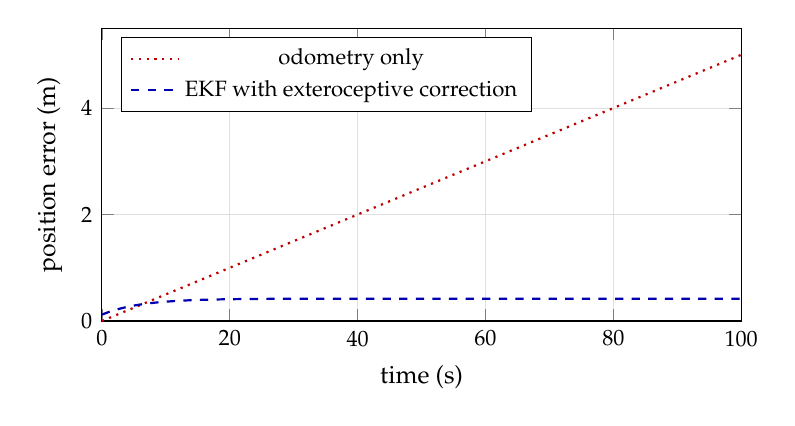
\begin{tikzpicture}
\begin{axis}[width=0.8\linewidth,height=5.3cm,xlabel={time (s)},ylabel={position error (m)},xmin=0,xmax=100,ymin=0,ymax=5.5,grid=both,grid style={gray!25},
  legend style={font=\footnotesize,at={(0.03,0.97)},anchor=north west},tick label style={font=\footnotesize},label style={font=\small}]
\addplot[thick,red!75!black,dotted,domain=0:100,samples=60] {0.05*x};
\addlegendentry{odometry only}
\addplot[thick,blue!70!black,dashed,domain=0:100,samples=100] {0.12+0.30*(1-exp(-x/6))};
\addlegendentry{EKF with exteroceptive correction}
\end{axis}
\end{tikzpicture}
\caption{Qualitative sketch (not experimental data): dead-reckoning error grows without bound, while with landmark or map measurements the EKF error remains bounded.}
\label{fig:errors}
\end{figure}

\subsection{Key take-aways}
\begin{itemize}
  \item \textbf{One loop, many sensors.} Localization with the EKF is always: predict with odometry ($\bm F_k$), compare the actual output with the predicted one (innovation $\bm\nu$, covariance $\bm S$), correct with the gain $\bm K$. Changing the sensor only changes $\bm h$ and its Jacobian $\bm H$.
  \item \textbf{Range--bearing landmarks:} $\bm h_i=(\rho,\beta)$ with $\bm H_i$ in closed form; position is observed by both components, while \emph{heading} is observed through the bearing (entry $-1$).
  \item \textbf{Unknown identity $\Rightarrow$ data association:} nearest neighbor with the Mahalanobis norm $\chi_{ij}=\bm\nu_{ij}^T\bm S_{ij}^{-1}\bm\nu_{ij}$, plus validation gating and mutual exclusion; it works only if the current estimate is already good.
  \item \textbf{Map-based localization} uses the whole scan, needs no explicit association, but suffers from aliasing; \textbf{SLAM} adds the landmark positions to the state (linear, hence a plain KF, for a point robot with ideal sensor) and trades a bigger state for not needing the map.
  \item \textbf{Gaussian beliefs are limited:} KF/EKF solve \emph{position tracking}; for the \emph{kidnapped robot} problem the belief is multimodal and particle filters are needed.
\end{itemize}

\end{document}